%==========================================================
%                 DEMONSTRAÇÃO DO TEMA FOCUS
%==========================================================
% Modificado por Gustavo Silva Rodrigues
% Instruções completas disponíveis em:
% https://github.com/gusirosx/Focus_theme
\documentclass[aspectratio=169]{beamer}
\usepackage[utf8]{inputenc}
\usepackage[T1]{fontenc} 
\usepackage{animate}
\usepackage[normalsize]{subfigure}
\usetheme{focus}
%==========================================================
%                 Configurações Iniciais
%==========================================================
\title{Demonstração do Tema Focus}
\subtitle{Um Tema Minimalista}
\author{Nome do Autor}
\institute{Universidade Federal de Uberlândia}
\titlegraphic{
\includegraphics[scale=0.12]{img/mflab.pdf}
	\hspace*{0.05cm}~
	
\includegraphics[scale=0.26]{img/petrobras.pdf}}
\date{Março de 2020}
%==========================================================
%                     Corpo do Documento
%==========================================================
% Adote boas práticas de programação e plante uma árvore
\begin{document}
%--------------------------------------------------------  
\begin{frame}
	\maketitle
\end{frame}
%--------------------------------------------------------    
\begin{frame}
	\frametitle{Conteúdo} 
	\tableofcontents 
\end{frame}
%========================================================
\section{Introdução}
%--------------------------------------------------------
\begin{frame}[plain, noframenumbering]{}
	\sectionpage
\end{frame}
%========================================================
\section{Parte 1}
%--------------------------------------------------------
\begin{frame}{Slide Simples}
	Esse é um Slide simples.
\end{frame}
%--------------------------------------------------------
\begin{frame}[plain]{Plain frame}
	Este é um slide com estilo simples e é numerado.
\end{frame}
%--------------------------------------------------------
\begin{frame}[t]
	Este slide tem um título vazio e está alinhado ao topo.
\end{frame}
%--------------------------------------------------------
\begin{frame}[noframenumbering]{Sem numeração de slides}
	Esse quadro não está numerado.
\end{frame}
%--------------------------------------------------------
\begin{frame}{Exemplo Prático 1}
	%\justifying
	Nas fronteiras o fluxo radiativo é avaliado por:
	\begin{equation}
	q_{rad_{w}} = - \frac{\varepsilon_w}{2(2 - \varepsilon_w)}\left[4\sigma T^{4}_{w} - G_w\right]
	\end{equation}
	Onde $\varepsilon_w$ é a emissividade na parede, considerando que para as fronteiras:
	\begin{equation}
	q_{rad_{w}} = - \Gamma \left.\frac{\partial G}{\partial n}\right|_w = -\Gamma\nabla G|_w
	\end{equation}
	Combinando as duas expressões, obtém-se a condição de contorno do modelo:
	\begin{equation}
	\Gamma\nabla G|_w + \theta G_w = 4\theta\sigma T^{4}_{w}
	\end{equation}
	Também conhecida como condição de Marshak, que é uma condição de 3ª espécie\footnote{Condição de Robin}.
\end{frame}
%--------------------------------------------------------
\begin{frame}{Exemplo Prático 2}
	\begin{figure}[!thp]
		\centering
		\subfigure[Before]{%
			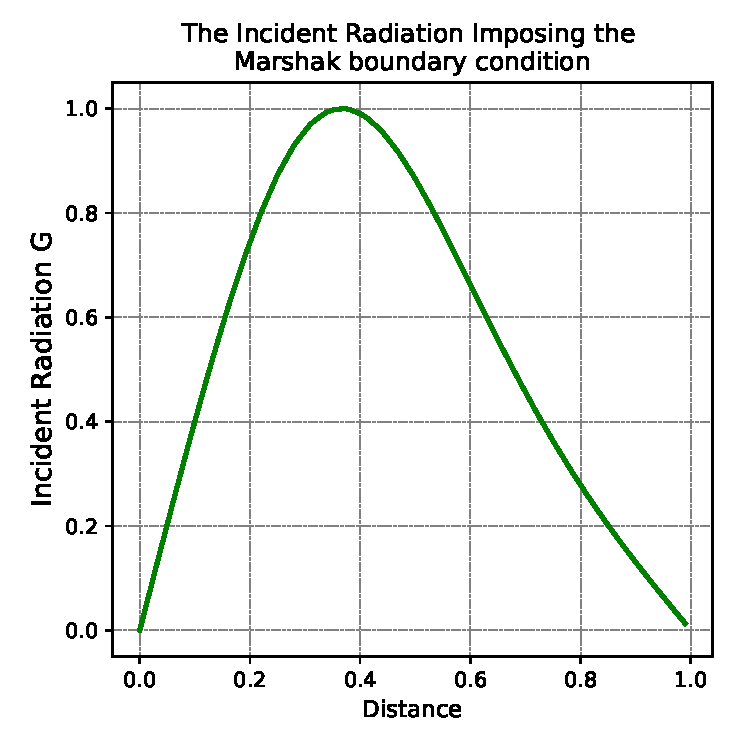
\includegraphics[width=0.45\textwidth]{./img/gw_d.pdf}%
		}\hfil
		\subfigure[Now]{%
			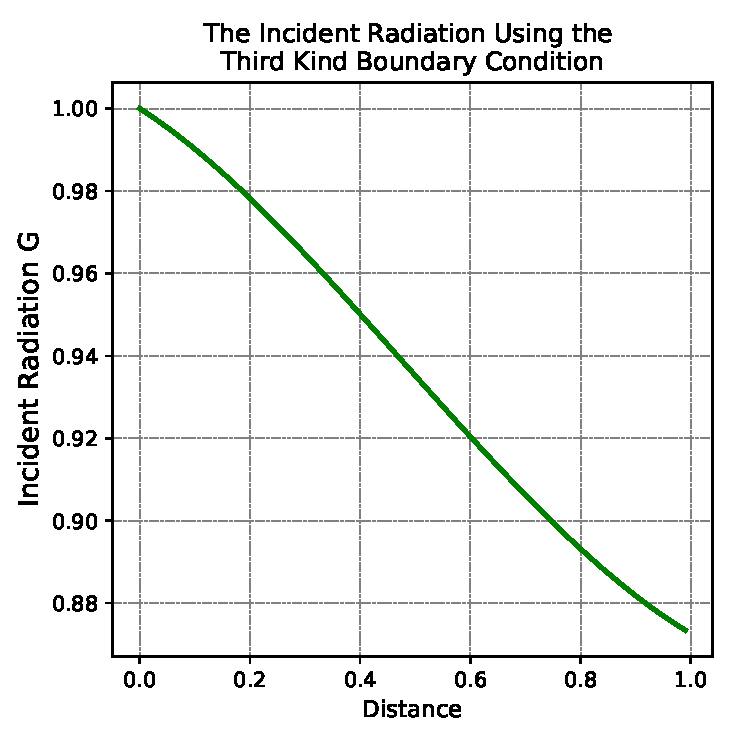
\includegraphics[width=0.45\textwidth]{./img/gw_thk.pdf}%
		}
		%\caption{}
	\end{figure}
\end{frame}
%--------------------------------------------------------
\begin{frame}{Tópicos}
	\vspace{-5cm}
	Etapas necessárias para o desenvolvimento desse projeto:
	\begin{enumerate}
		\item Etapa 1.
		\item Etapa 2.
		\item Etapa 3.
	\end{enumerate}
\end{frame}
%--------------------------------------------------------
\begin{frame}{Tipografia e Matemática}
	Os pacotes \texttt{inputenc} e \texttt{FiraSans}\footnote{\url{https://fonts.google.com/specimen/Fira+Sans}}\textsuperscript{,}\footnote{\url{http://mozilla.github.io/Fira/}} são utilizados para as fontes principais.
	\vfill
	Este tema fornece comandos de estilo ao digitar \alert{alertando}, \textbf{negrito}, \textcolor{example}{exemplo}, \dots
	\vfill
	\texttt{FiraSans} também fornece suporte para símbolos matemáticos:
	\begin{equation*}
	e^{i\pi} + 1 = 0.
	\end{equation*}
\end{frame}
%--------------------------------------------------------
\begin{frame}{Blocos}
	\begin{block}{Bloco}
		Texto.
	\end{block}
	\pause
	\begin{alertblock}{Bloco de Alerta}
		Alerta de \alert{Texto}.
	\end{alertblock}
	\pause
	\begin{exampleblock}{Bloco de Exemplo}
		Example \textcolor{example}{Texto}.
	\end{exampleblock}
\end{frame}
%--------------------------------------------------------
\begin{frame}{Listas}
	\begin{columns}[t, onlytextwidth]
		\column{0.33\textwidth}
		Itens:
		\begin{itemize}
			\item Item 1
			\begin{itemize}
				\item Subitem 1.1
				\item Subitem 1.2
			\end{itemize}
			\item Item 2
			\item Item 3
		\end{itemize}
		
		\column{0.33\textwidth}
		Enumerações:
		\begin{enumerate}
			\item Primeiro
			\item Segundo
			\begin{enumerate}
				\item Sub-primeiro
				\item Sub-segundo
			\end{enumerate}
			\item Terceiro
		\end{enumerate}
		
		\column{0.33\textwidth}
		Descrições:
		\begin{itemize}
			\item Primeiro \textcolor{example}{Sim}.
			\item Segundo \alert{Não}.
		\end{itemize}
	\end{columns}
\end{frame}
%--------------------------------------------------------
\setbeamertemplate{caption}[numbered]
\begin{frame}{Figures and Tables}
	\begin{columns}
		\column{0.4\textwidth}
         \begin{figure}
         	\centering
            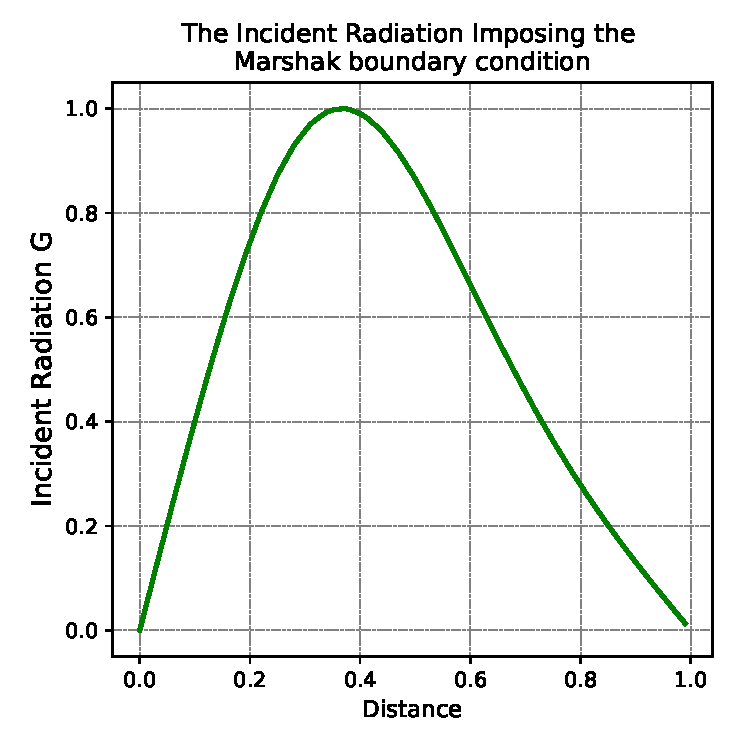
\includegraphics[width=0.8\textwidth]{./img/gw_d.pdf}
            \caption{Título.}
            \label{fig:focusl}
        \end{figure}    
        \column{0.6\textwidth}
        \begin{table}
       	\centering
        	\begin{tabular}{rcc}
            	& Coluna 1 & Coluna 2 \\\hline
                Linha 1 & \(v_{11}\) & \(v_{12}\) \\
                Linha 2 & \(v_{21}\) & \(v_{22}\) \\
               	Linha 3 & \(v_{31}\) & \(v_{32}\) \\
            \end{tabular}
        \caption{Título da tabela.}
        \label{tab:demo}
        \end{table}
    \end{columns}
\end{frame}
%--------------------------------------------------------
\begin{frame}[focus]
	Obrigado!
\end{frame}
%--------------------------------------------------------
\appendix
\begin{frame}{Referências}
    \nocite{*}
    \bibliography{bibliography}
	\bibliographystyle{plain}
\end{frame}
%--------------------------------------------------------
\begin{frame}{Slide Extra}
	\usebeamercolor[fg]{normal text}
	Esse é um slide de backup, útil para incluir material adicional para eventuais perguntas do público.
	\vfill
\end{frame}
%--------------------------------------------------------
\end{document}
